% SC4002 Chapter 3: Text Classification --- Naive Bayes, Logistic Regression, Transformers (0->100)
\chapter{Text Classification: Naive Bayes to Transformers}
\label{ch:classification}

\begin{quote}
\emph{``Classification is the task of choosing the right label for a piece of text. Every spam filter, sentiment analyser, and intent detector is a classifier.''} --- This chapter builds classifiers from counting words to attending with transformers.
\end{quote}

\noindent\fbox{\parbox{\dimexpr\linewidth-2\fboxsep-2\fboxrule}{%
\textbf{From zero: no ML background assumed.} We start from an email and a bag of words, then derive Naive Bayes from Bayes' rule, logistic regression from a linear boundary, and transformer classification from self-attention and a \texttt{[CLS]} token. Every formula is motivated by a picture first.}}
\vspace{0.4em}

\section*{Learning Outcomes}
After this chapter you will be able to:
\begin{enumerate}[label=(L\arabic*)]
    \item formulate text classification with bag-of-words and decision boundaries;
    \item derive and apply Naive Bayes with the conditional independence assumption;
    \item derive the logistic sigmoid, cross-entropy loss, and its gradient;
    \item explain transformer classification via self-attention and the \texttt{[CLS]} head;
    \item implement and fine-tune classifiers in Python.
\end{enumerate}

% ============================================================
\section{The Classification Problem}
\label{sec:classification-problem}
\paragraph{Intuition.} You open your inbox: ``WIN prize!!! Click now'' vs.\ ``Meeting at 3pm, room 101''. Without reading carefully you already guess spam or not from word clues. A classifier does exactly this---map a document $x$ to a label $y\in\{1,\dots,K\}$. The simplest representation forgets order: a \emph{bag-of-words} counts how often each vocabulary word occurs.

\paragraph{Formal setup.} Fix vocabulary $V=\{w_1,\dots,w_{|V|}\}$. Document $d$ becomes vector $\mathbf{x}\in\mathbb{N}^{|V|}$ with $x_j=\text{count}(w_j,d)$ (or TF-IDF weight). A dataset $\mathcal{D}=\{(\mathbf{x}^{(i)},y^{(i)})\}_{i=1}^N$ trains a function $f:\mathbb{N}^{|V|}\to\{1,\dots,K\}$. Visualise each document as a point; classification is drawing a boundary that separates colours (Fig.~\ref{fig:logistic-boundary}).

\paragraph{Example.} Vocabulary $\{\text{win},\text{prize},\text{meeting},\text{room}\}$. Email ``win prize win'' $\to [2,1,0,0]$, label spam ($y=1$). Email ``meeting room'' $\to [0,0,1,1]$, label ham ($y=0$). Even this tiny space already separates the two classes.

% ============================================================
\section{Naive Bayes: Counting with Bayes' Rule}
\label{sec:naive-bayes}
\paragraph{Intuition.} If 90\% of spam contains ``prize'' but only 2\% of ham does, seeing ``prize'' is strong evidence for spam. Naive Bayes inverts the direction: from $P(\text{words}\mid\text{class})$ to $P(\text{class}\mid\text{words})$.

\paragraph{Formal derivation.} Bayes' rule:
\begin{equation}
P(y\mid\mathbf{x})=\frac{P(y)\,P(\mathbf{x}\mid y)}{P(\mathbf{x})}\propto P(y)\prod_{j=1}^{|V|}P(w_j\mid y)^{x_j},
\label{eq:nb}
\end{equation}
where the \emph{Naive} step assumes words are conditionally independent given $y$. With Laplace smoothing $\alpha>0$:
\begin{equation}
P(w_j\mid y)=\frac{\text{count}(w_j,y)+\alpha}{\sum_{v}\text{count}(w_v,y)+\alpha|V|},\quad
\hat{y}=\arg\max_y \log P(y)+\sum_j x_j\log P(w_j\mid y).
\end{equation}
Training is counting; inference is a linear score in log-space.

\begin{figure}[h]
\centering
\begin{tikzpicture}[
  latent/.style={circle, draw=blue!60!black, thick, fill=blue!15, minimum size=9mm, font=\scriptsize},
  obs/.style={circle, draw=green!50!black, thick, fill=green!20, minimum size=9mm, font=\scriptsize},
  param/.style={circle, draw=orange!70!black, thick, fill=orange!15, minimum size=7mm, font=\tiny},
  plate/.style={draw=gray!60, thick, rounded corners=3pt, inner sep=6pt}
]
% Parameters
\node[param] (pi) at (0,2.2) {$\pi$};
\node[param] (phi) at (2.5,2.2) {$\phi$};
\node[font=\tiny, gray!60!black] at (0,2.75) {class prior};
\node[font=\tiny, gray!60!black] at (2.5,2.75) {word likelihoods};
% Class node
\node[latent] (y) at (0,0.9) {$y$};
% Word nodes
\node[obs] (w1) at (2.5,0.9) {$w_1$};
\node[obs] (w2) at (4.0,0.9) {$w_2$};
\node[font=\scriptsize, gray!60!black] at (5.1,0.9) {$\cdots$};
\node[obs] (wn) at (6.2,0.9) {$w_n$};
% Edges
\draw[-{Latex[length=2.2mm]}, thick, blue!60!black] (pi) -- (y);
\draw[-{Latex[length=2.2mm]}, thick, violet!70!black] (phi) -- (w1);
\draw[-{Latex[length=2.2mm]}, thick, violet!70!black] (phi) -- (w2);
\draw[-{Latex[length=2.2mm]}, thick, violet!70!black] (phi) -- (wn);
\draw[-{Latex[length=2.2mm]}, thick, blue!60!black] (y) -- (w1);
\draw[-{Latex[length=2.2mm]}, thick, blue!60!black] (y) -- (w2);
\draw[-{Latex[length=2.2mm]}, thick, blue!60!black] (y) -- (wn);
% Plates
\node[plate, fit=(w1)(w2)(wn), label={[font=\tiny, fill=orange!10, rounded corners=2pt, inner sep=2pt]south east:$n$ words}] (plateW) {};
\node[plate, fit=(y)(plateW), label={[font=\tiny, fill=blue!8, rounded corners=2pt, inner sep=2pt]south east:$N$ documents}] (plateD) {};
% Legend
\node[font=\tiny, align=left, fill=yellow!8, draw=gray!40, rounded corners=2pt, inner sep=3pt] at (3.0,-0.85) {\textcolor{blue!60!black}{$\blacksquare$ latent} \ \textcolor{green!50!black}{$\blacksquare$ observed} \ \textcolor{orange!70!black}{$\blacksquare$ parameter} \ \ \textcolor{violet!70!black}{$\rightarrow$ generative link}};
\end{tikzpicture}
\caption{Naive Bayes generative plate diagram. For each document, sample class $y\sim\text{Cat}(\pi)$, then each word $w_i\sim\text{Cat}(\phi_y)$ independently given $y$. Plates replicate over words ($n$) and documents ($N$). Despite the independence assumption, NB is a strong baseline for spam and topic classification.}
\label{fig:nb-plate}
\end{figure}

Fig.~\ref{fig:nb-plate} shows the generative story. Learning estimates $\pi$ and $\phi$ by counts; classification applies Eq.~\eqref{eq:nb}. Smoothing prevents zero probabilities for unseen word--class pairs.

% ============================================================
\section{Logistic Regression: A Linear Boundary with Probabilities}
\label{sec:logistic}
\paragraph{Intuition.} Naive Bayes is generative (models how data is created). Logistic regression is \emph{discriminative}: draw a straight line (hyperplane) between classes and squash its distance into a probability. Points far on one side are confidently spam.

\paragraph{Formal model.} For binary $y\in\{0,1\}$ with features $\mathbf{x}\in\mathbb{R}^d$:
\begin{equation}
P(y=1\mid\mathbf{x})=\sigma(\mathbf{w}^\top\mathbf{x}+b),\quad \sigma(z)=\frac{1}{1+e^{-z}}\in(0,1).
\end{equation}
Decision boundary is $\mathbf{w}^\top\mathbf{x}+b=0$ (where $P=0.5$). Training minimises cross-entropy:
\begin{equation}
\mathcal{L}(\mathbf{w},b)=-\frac1N\sum_{i=1}^N\Big[y^{(i)}\log\hat{y}^{(i)}+(1-y^{(i)})\log(1-\hat{y}^{(i)})\Big],\ \ \hat{y}^{(i)}=\sigma(\mathbf{w}^\top\mathbf{x}^{(i)}+b).
\end{equation}
Gradient (derived via chain rule, $\sigma'(z)=\sigma(z)(1-\sigma(z))$):
\begin{equation}
\nabla_{\mathbf{w}}\mathcal{L}=\frac1N\sum_{i=1}^N(\hat{y}^{(i)}-y^{(i)})\mathbf{x}^{(i)},\quad
\frac{\partial\mathcal{L}}{\partial b}=\frac1N\sum_i(\hat{y}^{(i)}-y^{(i)}).
\end{equation}
Update: $\mathbf{w}\gets\mathbf{w}-\eta\nabla_{\mathbf{w}}\mathcal{L}$. No closed form---optimise by gradient descent.

\begin{figure}[h]
\centering
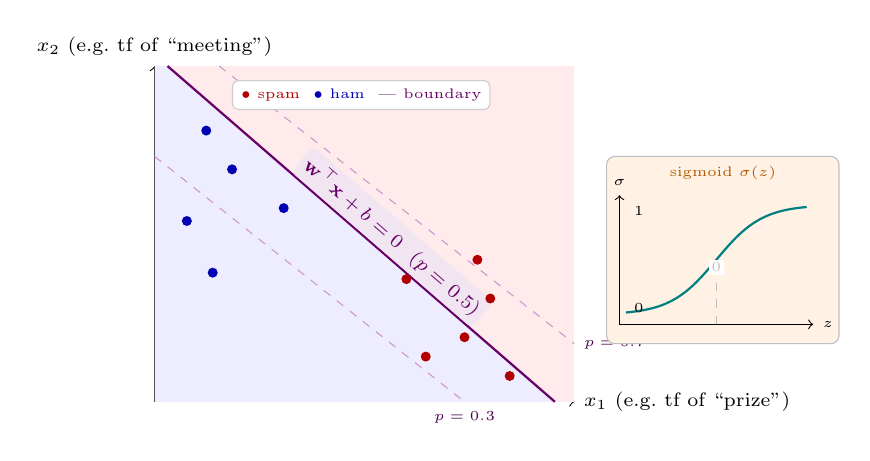
\begin{tikzpicture}[scale=0.82, every node/.style={font=\scriptsize}]
% Axes
\draw[->] (0,0) -- (6.5,0) node[right] {$x_1$ (e.g.\ tf of ``prize'')};
\draw[->] (0,0) -- (0,5.2) node[above] {$x_2$ (e.g.\ tf of ``meeting'')};
% Background shading
\fill[red!8] (0,0) rectangle (6.5,5.2);
\fill[blue!7] (0,0) -- (6.2,0) -- (0.2,5.2) -- (0,5.2) -- cycle;
% Decision boundary
\draw[thick, violet!80!black] (0.2,5.2) -- (6.2,0) node[pos=0.55, above, sloped, fill=violet!10, rounded corners=2pt, inner sep=2pt] {$\mathbf{w}^\top\mathbf{x}+b=0$ \ ($p=0.5$)};
% Probability contours
\draw[violet!40, dashed] (1.0,5.2) -- (6.5,0.9) node[right, font=\tiny, violet!60!black] {$p=0.7$};
\draw[violet!40, dashed] (0,3.8) -- (4.8,0) node[below, font=\tiny, violet!60!black] {$p=0.3$};
% Spam points (red)
\foreach \x/\y in {4.8/1.0,5.2/1.6,4.2/0.7,5.5/0.4,3.9/1.9,5.0/2.2} \fill[red!70!black] (\x,\y) circle (2.2pt);
% Ham points (blue)
\foreach \x/\y in {0.8/4.2,1.2/3.6,0.5/2.8,1.5/4.7,2.0/3.0,0.9/2.0} \fill[blue!70!black] (\x,\y) circle (2.2pt);
% Sigmoid inset
\begin{scope}[shift={(7.2,1.2)}]
  \draw[fill=orange!10, rounded corners=3pt, draw=gray!50] (-0.2,-0.3) rectangle (3.4,2.6);
  \node[font=\tiny, orange!70!black] at (1.6,2.35) {sigmoid $\sigma(z)$};
  \draw[->] (0,0) -- (3.0,0) node[right, font=\tiny] {$z$};
  \draw[->] (0,0) -- (0,2.0) node[above, font=\tiny] {$\sigma$};
  \draw[teal, thick] plot[domain=-1.4:1.4, smooth, samples=40] ({\x+1.5},{1.0+0.85*tanh(1.4*\x)});
  \draw[gray!50, dashed] (1.5,0) -- (1.5,1.0) node[below, font=\tiny, fill=white, inner sep=1pt] {$0$};
  \node[font=\tiny] at (0.3,1.75) {$1$}; \node[font=\tiny] at (0.3,0.25) {$0$};
\end{scope}
% Legend
\node[font=\tiny, align=left, fill=white, draw=gray!40, rounded corners=2pt, inner sep=3pt] at (3.2,4.75) {\textcolor{red!70!black}{$\bullet$ spam} \ \textcolor{blue!70!black}{$\bullet$ ham} \ \textcolor{violet!80!black}{--- boundary}};
\end{tikzpicture}
\caption{Logistic regression as a linear decision boundary. Background tint shows predicted $P(y=1\mid\mathbf{x})$; dashed lines are probability contours. Inset: sigmoid $\sigma(z)$ squashes the linear score $z=\mathbf{w}^\top\mathbf{x}+b$ into $(0,1)$.}
\label{fig:logistic-boundary}
\end{figure}

% ============================================================
\section{Transformers for Classification}
\label{sec:transformer-cls}
\paragraph{Intuition.} Bag-of-words ignores order: ``dog bites man'' vs.\ ``man bites dog'' look identical. Transformers read the whole sentence at once, letting every word attend to every other word, then summarise the sentence into one vector for classification.

\paragraph{Formal mechanism.} Input tokens $[ \text{[CLS]}, w_1,\dots,w_n, \text{[SEP]}]$ are embedded $\mathbf{E}\in\mathbb{R}^{(n+2)\times d}$. Each layer computes self-attention:
\begin{equation}
\text{Attn}(Q,K,V)=\text{softmax}\!\left(\frac{QK^\top}{\sqrt{d_k}}\right)V,\quad Q=\mathbf{E}W_Q,\ K=\mathbf{E}W_K,\ V=\mathbf{E}W_V,
\end{equation}
with multi-head concatenation and feed-forward sublayers. After $L$ layers, the \texttt{[CLS]} vector $\mathbf{h}_{\text{[CLS]}}\in\mathbb{R}^d$ is a contextual summary. A classification head projects it:
\begin{equation}
\mathbf{logits}= \mathbf{h}_{\text{[CLS]}}W_c+\mathbf{b}_c,\quad P(y\mid\mathbf{x})=\text{softmax}(\mathbf{logits})_y.
\end{equation}
Fine-tuning updates all weights (or just the head) by cross-entropy, using the \texttt{[CLS]} hidden state as the sentence vector---no manual features needed.

\begin{figure}[h]
\centering
\begin{tikzpicture}[
  tok/.style={draw=blue!60!black, thick, fill=blue!12, minimum width=1.15cm, minimum height=0.65cm, font=\scriptsize, rounded corners=2pt},
  cls/.style={draw=violet!70!black, thick, fill=violet!15, minimum width=1.15cm, minimum height=0.65cm, font=\scriptsize, rounded corners=2pt},
  hid/.style={draw=teal!60!black, thick, fill=teal!15, minimum width=1.15cm, minimum height=0.65cm, font=\scriptsize, rounded corners=2pt},
  attn/.style={-{Latex[length=1.8mm]}, thin, orange!70!black, opacity=0.55},
  head/.style={draw=orange!70!black, thick, fill=orange!15, rounded corners=3pt, minimum height=0.7cm, font=\scriptsize}
]
% Input tokens
\node[cls] (t0) at (0,0) {[CLS]};
\node[tok] (t1) at (1.7,0) {win};
\node[tok] (t2) at (3.4,0) {prize};
\node[tok] (t3) at (5.1,0) {now};
\node[tok] (t4) at (6.8,0) {[SEP]};
\node[font=\tiny, gray!60!black] at (3.4,-0.55) {input embeddings + positional encoding};
% Hidden states
\node[hid] (h0) at (0,2.0) {$\mathbf{h}_{\text{CLS}}$};
\node[hid] (h1) at (1.7,2.0) {$\mathbf{h}_1$};
\node[hid] (h2) at (3.4,2.0) {$\mathbf{h}_2$};
\node[hid] (h3) at (5.1,2.0) {$\mathbf{h}_3$};
\node[hid] (h4) at (6.8,2.0) {$\mathbf{h}_4$};
\node[font=\tiny, gray!60!black] at (3.4,2.65) {$L$ transformer layers (self-attention $\times$ heads)};
% Attention arrows (all to all, faint)
\foreach \s in {0,1,2,3,4} \foreach \t in {0,1,2,3,4} \draw[attn] (t\s.north) -- (h\t.south);
% Transformer block
\node[draw=gray!50, thick, fill=gray!5, rounded corners=4pt, fit=(h0)(h4), inner sep=6pt, label={[font=\tiny, fill=teal!10, rounded corners=2pt, inner sep=2pt]north:Transformer encoder}] (enc) {};
% Classification head
\node[head, minimum width=2.4cm] (clf) at (0,3.7) {Linear $W_c$ + softmax};
\draw[-{Latex[length=2.5mm]}, thick, violet!70!black] (h0.north) -- (clf.south) node[midway, right, font=\tiny, fill=violet!10, rounded corners=2pt, inner sep=2pt] {CLS only};
% Output
\node[draw=green!50!black, thick, fill=green!15, rounded corners=3pt, minimum width=2.4cm, minimum height=0.6cm, font=\scriptsize] (out) at (0,4.85) {$P(y\mid\mathbf{x})$};
\draw[-{Latex[length=2.5mm]}, thick, green!50!black] (clf.north) -- (out.south);
% Legend
\node[font=\tiny, align=left, fill=yellow!8, draw=gray!40, rounded corners=2pt, inner sep=3pt] at (4.8,4.55) {\textcolor{orange!70!black}{$\rightarrow$ attention} \ \textcolor{violet!70!black}{$\rightarrow$ CLS path}};
\end{tikzpicture}
\caption{Transformer classification head. All tokens attend to all others through $L$ layers; only $\mathbf{h}_{\text{[CLS]}}$ feeds the classifier. Fine-tuning adjusts $W_Q,W_K,W_V$ and $W_c$ jointly via cross-entropy on $P(y\mid\mathbf{x})$.}
\label{fig:transformer-cls}
\end{figure}

\begin{lstlisting}[language=Python, caption={Naive Bayes from scratch (counts + Laplace) and transformer fine-tuning with Hugging Face.}, label={lst:nb-transformer}]
import numpy as np
from collections import Counter, defaultdict

# --- Naive Bayes from scratch ---
docs = [("win prize win", 1), ("win free prize", 1), ("meeting room today", 0),
        ("room meeting tomorrow", 0), ("free win prize", 1), ("today meeting", 0)]
vocab = sorted({w for d,_ in docs for w in d.split()})
V, alpha = len(vocab), 1.0
counts = {0: Counter(), 1: Counter()}
priors = Counter(y for _, y in docs)
for text, y in docs:
    counts[y].update(text.split())

def predict(text):
    words = text.split()
    scores = {}
    for y in [0, 1]:
        logp = np.log(priors[y] / len(docs))
        total = sum(counts[y].values())
        for w in words:
            pw = (counts[y][w] + alpha) / (total + alpha * V)
            logp += np.log(pw)
        scores[y] = logp
    return max(scores, key=scores.get), scores

print(predict("free prize"))   # -> (1, {0: -7.1, 1: -3.8}) spam wins
print(predict("meeting today"))  # -> (0, ...) ham wins

# --- Fine-tune BERT for classification (Hugging Face) ---
# pip install transformers datasets
from transformers import AutoTokenizer, AutoModelForSequenceClassification, Trainer, TrainingArguments
from datasets import Dataset

raw = Dataset.from_list([{"text": d, "label": y} for d, y in docs * 20])
tok = AutoTokenizer.from_pretrained("distilbert-base-uncased")
def tokenize(b): return tok(b["text"], truncation=True, padding="max_length", max_length=16)
ds = raw.map(tokenize, batched=True).train_test_split(test_size=0.2)

model = AutoModelForSequenceClassification.from_pretrained(
    "distilbert-base-uncased", num_labels=2)
args = TrainingArguments(output_dir="./bert-cls", per_device_train_batch_size=8,
                         num_train_epochs=3, learning_rate=2e-5, logging_steps=5)
Trainer(model=model, args=args, train_dataset=ds["train"],
        eval_dataset=ds["test"], tokenizer=tok).train()
\end{lstlisting}

% ============================================================
\section{Chapter Notes}
Naive Bayes dates to the 1960s spam filters; despite independence being false, it remains competitive on small data. Logistic regression (Cox, 1958) is the discriminative counterpart---same linear form, different training objective. Transformers for classification were popularised by BERT \cite{devlin2019bert}: the \texttt{[CLS]} trick turns any encoder into a classifier by fine-tuning. For deeper theory see Bishop Ch.~4 (generative vs.\ discriminative) and Jurafsky \& Martin Ch.~4--11.

% ============================================================
\section{Exercises}
\label{sec:ch03-exercises}
\begin{enumerate}[label=E3.\arabic*, leftmargin=*, itemsep=0.7em]
    \item \textbf{NB by hand.} With the six documents above and $\alpha=1$, compute $P(\text{``prize''}\mid y=1)$, $P(\text{``meeting''}\mid y=0)$, and $P(y=1\mid\text{``win meeting''})$ via Eq.~\eqref{eq:nb}. Show smoothing changes the result vs.\ $\alpha=0$.
    \item \textbf{Decision boundary.} Let $\mathbf{w}=[2,-1]^\top$, $b=-1$. (a) Sketch $\mathbf{w}^\top\mathbf{x}+b=0$ for $\mathbf{x}\in\mathbb{R}^2$ and label the $p>0.5$ side. (b) Compute $\sigma(\mathbf{w}^\top\mathbf{x}+b)$ for $\mathbf{x}=[1,1]^\top$ and $[3,0]^\top$. (c) Explain why logistic regression cannot separate XOR points $\{(0,0),(1,1)\}$ vs.\ $\{(0,1),(1,0)\}$.
    \item \textbf{Gradient step.} For one example $\mathbf{x}=[1,2]^\top$, $y=1$, current $\mathbf{w}=[0,0]^\top$, $b=0$, compute $\hat{y}$, the loss, and one SGD step with $\eta=0.5$. Repeat for $y=0$.
    \item \textbf{CLS vs.\ pooling.} A colleague averages all $\mathbf{h}_i$ instead of using $\mathbf{h}_{\text{[CLS]}}$ for classification. (a) Give one advantage of \texttt{[CLS]} (hint: pre-training objective). (b) Describe a case where mean-pooling might help. (c) How does self-attention ensure $\mathbf{h}_{\text{[CLS]}}$ still sees every word?
    \item \textbf{Build and compare.} Extend the NB code to (a) use TF-IDF weights instead of counts, (b) evaluate accuracy on a held-out split, and (c) compare against \texttt{sklearn.linear\_model.LogisticRegression} and the fine-tuned DistilBERT. Report which wins on 6 vs.\ 600 documents and explain why.
\end{enumerate}
% End of Chapter 3